\documentclass[18pt]{beamer}
%% SLIDE FORMAT
\usepackage[utf8]{inputenc}
\usepackage{algpseudocode}



\title[Programmieren Tutorium]{5. Programmieren Tutorium:\texorpdfstring{\\}{} Warum Objektorientierung?}
\subtitle{Sichtbarkeiten}
\author{Konstantin Zangerle \texorpdfstring{\\}{} info@konstantinzangerle.de}
\date{30. Nov 2015}

\usepackage{listings}
\usepackage{color}

\definecolor{mygreen}{rgb}{0,0.6,0}
\definecolor{mygray}{rgb}{0.5,0.5,0.5}
\definecolor{mymauve}{rgb}{0.58,0,0.82}

\lstset{ %
  backgroundcolor=\color{white},   % choose the background color
  basicstyle=\footnotesize,        % size of fonts used for the code
  breaklines=true,                 % automatic line breaking only at whitespace
  captionpos=b,                    % sets the caption-position to bottom
  commentstyle=\color{mygreen},    % comment style
  escapeinside={\%*}{*)},          % if you want to add LaTeX within your code
  keywordstyle=\color{blue},       % keyword style
  stringstyle=\color{mymauve},     % string literal style
  showstringspaces=false,
  language=Java
}
\beamersetuncovermixins{\opaqueness<1>{0}}{\opaqueness<2->{0}} %Dont show things after pause 
% Bibliography

\begin{document}

% change the following line to "ngerman" for German style date and logos
\selectlanguage{ngerman}

%title page
\begin{frame}
\titlepage
\end{frame}

%table of contents
\begin{frame}{Gliederung}
\tableofcontents
\end{frame}

\section{Übungsblatt}

\subsection{Statistik}
\begin{frame}{Statistik Übungsblatt 1}
\begin{itemize}
 \item Teil A: 1.45 vs 1,55 von 2 
 \item Teil B: 1.77 vs 1,64 von 2 	
 \item Teil C: 1,95 vs 1,70 von 2 	
 \item Teil D: 5,95 vs 5,74 von 7	
 \item Teil E: 2,77 vs 2,55 von 3
 \item Teil F: 1,64 vs 1,66 von 2
 \item Teil G: 1,9 vs 1,61 von 2
\end{itemize}
So weit also gut :)
\end{frame}


\section{Rückblick}
\begin{frame}{Rückblick}
 \begin{itemize}
  \item Attribute
  \item Variablen
  \item Datentypen
  \item Methoden
  \item Kontrollstrukturen
  \item Arrays
  \item Checkstyle
  \item Präzedenz
  \item String
  \item Referenzen
 \end{itemize}
\end{frame}

\section{Heute + nächste Woche}
\begin{frame}[fragile]{Ausblick}
\begin{itemize}
 \item Vererbung
 \item Dynamische Bindung
 \item Überschreibung von Attributen und Methoden
 \item Konstruktoren mit \verb|super|
 \item Typumwandlungen
 \item Klasse \verb|Object| und Java-Klassenhierarchie
 \item Abstrakte Klassen
 \item Inhaltliche Gleichheit
 \item \verb|final|
 \item Javadoc
 \item Verkette Listen und Iteratoren
 \item Queue, Stack, Priority Queue
 \item Schnittstellen
 \item Generische Klassen und Schnittstellen
  \item \verb|instanceof|
\end{itemize}
\end{frame}

\begin{frame}[fragile]{Heute}
\begin{itemize}
 \item Vererbung
 \item Überschreibung von Attributen und Methoden
 \item Generische Klassen und Schnittstellen
 \item Javadoc
 \item Konstruktoren mit \verb|super|
 \item Schnittstellen 
\end{itemize}
\end{frame}

\section{Arrays} % 4-7


\begin{frame}[fragile]{Arrays}
 \begin{lstlisting}
    public static int max(int[] a) {
        int max = Integer.MIN_VALUE;
        for (int k : a) {
            if (k >= max) {
                max = k;
            }
        }
        return max;
    }
 \end{lstlisting}
\end{frame}

\begin{frame}{Arrays – Was muss man beachten}
 \begin{itemize}
  \item Arrays sollen Daten zusammenfassen, die zusammengehören
  \item Auch wenns geht, so ein Array ist blöd [Handelsklasse, Gewicht, Volumen, Gewicht]
  \item Eignen sich für feste Datengrößen (5x int; double-Feld 5x3; ...)
 \end{itemize}

\end{frame}

\subsection{Sichtbarkeit}
\begin{frame}[fragile]{Sichtbarkeit}
 Um Programmierer dazu zu zwingen, die Datenkapselung einzuhalten,
 benutzen wir Sichtbarkeiten. Ist ein Attribut oder eine Methode als 
 \verb|private| gekennzeichent, so ist ein Zugriff nur innerhalb
 derselben Klasse möglich.
 Es gibt (in Java) drei Sichtbarkeiten:
 \begin{itemize}
  \item public
  \item protected
  \item private
 \end{itemize}
\end{frame}

\subsection{Packages}
\section{Graphentheorie}
\begin{frame}{Was ist ein Graph?}
 Schwierige Frage.
 \begin{itemize}
  \item Eine Zeichnung mit Knoten und Kanten 
  \item Eine Operation auf einer Menge. 
  \item Eine Veranschaulichung einer Relation 
 \end{itemize}
\end{frame}

\subsection{Darstellung als Arrays}
\begin{frame}{Graphen als Arrays}
Kommt genauer im zweiten Semester. Hier dürft ihr das machen.
Ihr benötigt zwei Arrays. Eine speichert, wie viele Kanten von einer
Kante ausgehen. Die andere speichert die Ziele der Kanten.

\textbf{Aufgabe:} Entwerfe eine Klasse Graph, die einen Graphen speichern
kann. Die Knoten sollen hierbei von 0 durchnummeriert werden.
\end{frame}


\section{Packages}
\subsection{Definitionen}
\begin{frame}{Packages}
 Sind die Module in Java. \pause
 
 \begin{exampleblock}{Definition: Modul}
  Ein Modul (neutrum, das Modul[1]) ist eine abgeschlossene funktionale Einheit einer Software, 
  bestehend aus einer Folge von Verarbeitungsschritten und Datenstrukturen. Inhalt eines Moduls ist
  häufig eine wiederkehrende Berechnung oder Bearbeitung von Daten, die mehrfach durchgeführt 
  werden muss. Das Modul führt eine Reihe von Verarbeitungsschritten durch, liefert bei der 
  Rückkehr an das aufrufende Programm Daten als Ergebnis zurück.
  
  \tiny{Quelle: http://de.wikipedia.org/wiki/Modul\_\%28Software\%29 }
 \end{exampleblock}

\end{frame}

\begin{frame}{Packages}
 Sind die Module in Java. \pause
 
 \begin{exampleblock}{Definition: Modul (SWT)}
 Ein Modul ist eine Menge von Programmelementen, die nach dem Geheimnisprinzip gemeinsam entworfen und geändert werden.

 \end{exampleblock}

\end{frame}

\begin{frame}{Packages}
\tiny
A package is a namespace that organizes a set of related classes and interfaces. 
Conceptually you can think of packages as being similar to different folders on your computer. 
You might keep HTML pages in one folder, images in another, and scripts or applications in yet another. 
Because software written in the Java programming language can be composed of hundreds or thousands of 
individual classes, it makes sense to keep things organized by placing related classes and interfaces into packages.

The Java platform provides an enormous class library (a set of packages) suitable for use in your own 
applications. This library is known as the ``Application Programming Interface'', or ``API'' for short. 
Its packages represent the tasks most commonly associated with general-purpose programming. For example, 
a String object contains state and behavior for character strings; a File object allows a programmer to easily 
create, delete, inspect, compare, or modify a file on the filesystem; a Socket object allows for the creation
and use of network sockets; various GUI objects control buttons and checkboxes and anything else related to 
graphical user interfaces. There are literally thousands of classes to choose from. This allows you, the programmer, 
to focus on the design of your particular application, rather than the infrastructure required to make it work.

\emph{The Java Platform API Specification contains the complete listing for all packages, interfaces, classes, fields, 
and methods supplied by the Java SE platform. Load the page in your browser and bookmark it. As a programmer, 
it will become your single most important piece of reference documentation.}

\end{frame}

\begin{frame}{Packages}
\scriptsize
A package is a namespace that organizes a set of related classes and interfaces. 
Conceptually you can think of packages as being similar to different folders on your computer. 
You might keep HTML pages in one folder, images in another, and scripts or applications in yet another. 
Because software written in the Java programming language can be composed of hundreds or thousands of 
individual classes, it makes sense to keep things organized by placing related classes and interfaces into packages.

The Java platform provides an enormous class library (a set of packages) suitable for use in your own 
applications. This library is known as the ``Application Programming Interface'', or ``API'' for short. 
Its packages represent the tasks most commonly associated with general-purpose programming. For example, 
a String object contains state and behavior for character strings; a File object allows a programmer to easily 
create, delete, inspect, compare, or modify a file on the filesystem; a Socket object allows for the creation
and use of network sockets; various GUI objects control buttons and checkboxes and anything else related to 
graphical user interfaces. There are literally thousands of classes to choose from. This allows you, the programmer, 
to focus on the design of your particular application, rather than the infrastructure required to make it work.

\emph{The Java Platform API Specification contains the complete listing for all packages, interfaces, classes, fields, 
and methods supplied by the Java SE platform. Load the page in your browser and bookmark it. As a programmer, 
it will become your single most important piece of reference documentation.}

\end{frame}

\begin{frame}{Packages}
\begin{alertblock}{Wichtig}
\Large
\emph{The Java Platform API Specification contains the complete listing for all packages, interfaces, classes, fields, 
and methods supplied by the Java SE platform. Load the page in your browser and bookmark it. As a programmer, 
it will become your single most important piece of reference documentation.}
 
\end{alertblock}

\end{frame}

\section{Listen}

\subsection{Iterator}

\subsection{Vgl. Array und Listen}



\section{Vererbung}
\subsection{Einführung}
\begin{frame}{Vererbung}
 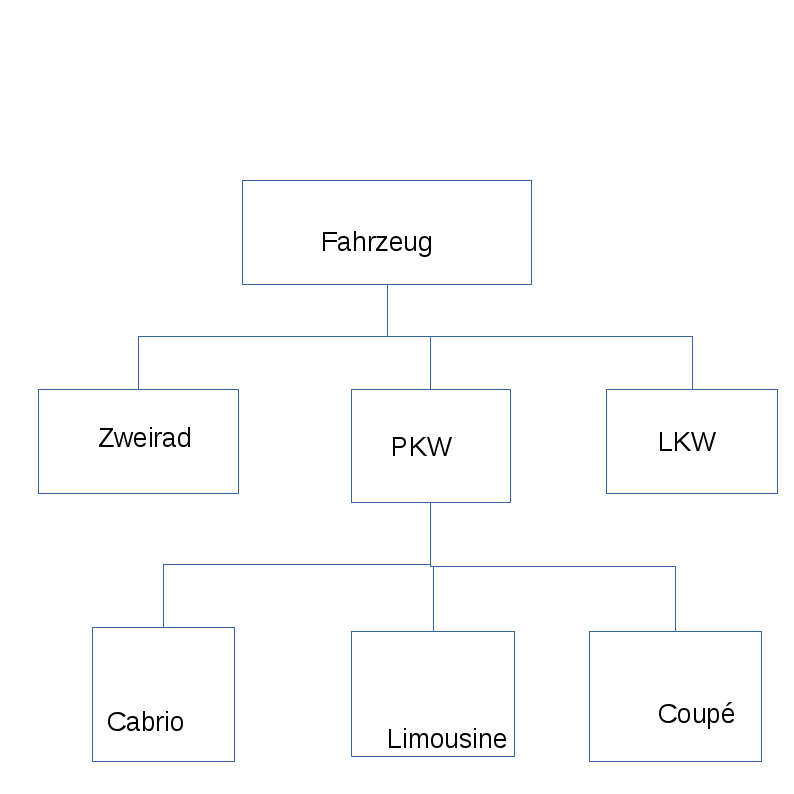
\includegraphics[scale=0.25]{Fahrzeuge.png}
 \begin{itemize}
 \item Ein PKW ist ein Fahrzeug, ein Zweirad ist ein Fahrzeug, 
  \item Eine Limousine ist ein Fahrzeug, aber nicht jedes Fahrzeug ist eine Limousine
  \item Jedes Cabrio kann das Dach öffnen bzw. schließen, bei PKWs macht das (meistens) keinen Sinn.
 \end{itemize}
\end{frame}

\begin{frame}{Genauer: Vererbung}
 \begin{itemize}
  \item Vererbung ist eine ``ist''-Beziehung
  \item Alle Eigenschaften (Attribute) werden übernommen!
  \item Alle Methoden werden übernommen.
  \item Kinder haben aber auch Freiheiten diese zu ändern!
 \end{itemize}
\end{frame}


\subsection{In Java?!}
\begin{frame}[fragile]{In Java!}
 \begin{enumerate}
  \item Überlege welche Klassen du benötigst
  \item Überlege welche sinnvollen Vererbungsbeziehungen du aufstellen kannst!
  \item Erstelle jede Klasse ``normal''.
  \item Benutze \verb|public class X extends Schinken {|
 \end{enumerate}
\end{frame}

\subsection{Aufgabe zur Vererbung}
\begin{frame}{Übung!}
 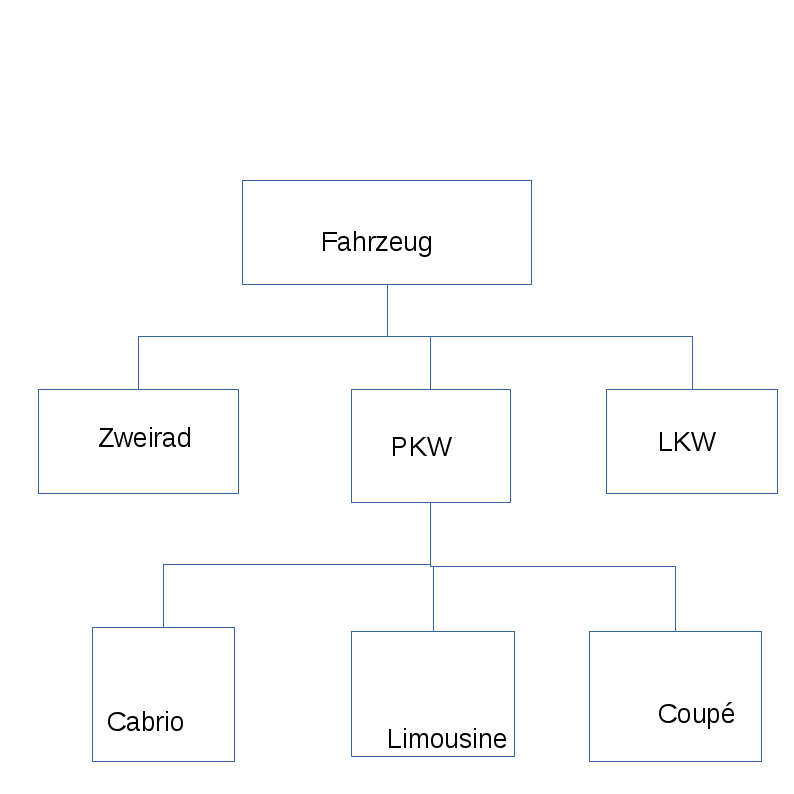
\includegraphics[scale=0.25]{Fahrzeuge.png}
 \begin{itemize}
  \item Modelliere den Abschnitt PKW, Cabrio, Limousine, Coupé
  \item Füge sinnvolle Attribute in sinnvollen Klassen hinzu!
  \item Füge sinnvolle Methoden in sinnvollen Klassen hinzu!
  \item Benutze Vererbung!
 \end{itemize}

\end{frame}


\section{Methoden und Methoden in Vererbung}
\begin{frame}[fragile]{Überschreibung von Methoden}
Betrachte die Klassen
\begin{lstlisting}
public class Motor {
  public void starten() { ... }
}

public class DieselMotor extends Motor {
  @Override
  public void starten() { ... }
} 
\end{lstlisting}
\pause
\begin{itemize}
 \item Warum ist diese Vererbung sinnvoll? \pause
 \item Warum sollte man die starten Methode überschreiben? \pause
 \item Warum steht hier @Override? \pause
 \item Warum liegt hier überhaupt Stroh rum?
\end{itemize}
\end{frame}

\begin{frame}{Aufgabe}
 \begin{itemize}
  \item Jeder (funktionierende) PKW hat ein Motor? Oder?
  \item Wenn dem so ist, füge dies als Attribut hinzu.
  \item Schreibe einen Konstruktor, der ein Motorobjekt annimmt und diesen an die super-Klasse PKW weitergibt.
 \end{itemize}
\end{frame}

\begin{frame}[fragile]{Überschatten von Attributen}
 \begin{lstlisting}
  class SuperBoaster {
  int nr = 1;
  void boast()  {
    System.out.println( "Ich bin die Nummber " + nr );
  }
}
public class SubBoaster extends SuperBoaster {
  int nr = 2;
  @Override 
  void boast()  {
    super.boast();                   // Ich bin die Nummber 1
    System.out.println( super.nr );  // 1
    System.out.println( nr );        // 2
  }

  public static void main( String[] args )  {
    new SubBoaster().boast();
  }
} //Geklaut von: Java ist auch eine Insel 5.11.5
 \end{lstlisting}
\end{frame}


\begin{frame}{Konstruktoren und super}
 \begin{alertblock}{Ein wichtiger Unterschied}
  In Konstruktoren muss der super() Konstruktor als erstes aufgerufen werden,
  oder gar nicht!
 \end{alertblock}
\end{frame}


\begin{frame}[fragile]{Generische Klassen}
 \begin{lstlisting}
  ArrayList<String> liste = new ArrayList<String>(); //oder...
  Liste liste = new ArrayList<String>();
 \end{lstlisting}
\end{frame}


\begin{frame}[fragile]{Schnittstellen}
\begin{lstlisting}
 interface Motor {
  public void starten();
  public int getLeistung();
 }
 \end{lstlisting}
 \begin{itemize}
  \item Interfaces stellen eine Schablone dar.
  \item Interfaces geben die Gewissheit, das Klassen, die diese implementieren, Funktionen besitzen.
  \item Interfaces haben keine Attribute.
 \end{itemize}

\end{frame}

\begin{frame}[fragile]{Javadoc}
 Javadoc sind Kommentare mit folgendem Schema:
 \begin{lstlisting}
  /**
 * Kurzbeschreibung der Funktionalitaet in einem Satz.
 * Weitere Details folgen darauf.
 * 
 * Beschreibung von Parametern, Rueckgabewerten und co.
 * geschieht durch spezielle Tags.
 */
 \end{lstlisting}
Außerdem können ``Tags'' verwendet werden, bspw. @author, @version, @param, @return, @throws
Siehe dazu den Eintrag im Programmieren Wiki
\scriptsize
\verb|https://ilias.studium.kit.edu/goto.php?target=wiki_349162_Javadoc|
\end{frame}


\section{ToDo-Liste}
\begin{frame}[fragile]{ToDo-Liste}
\begin{itemize}
 \item Vererbung \checkmark
 \item Dynamische Bindung
 \item Überschreibung von Attributen und Methoden \checkmark
 \item Konstruktoren mit \verb|super| \checkmark
 \item Typumwandlungen 
 \item Klasse \verb|Object| und Java-Klassenhierarchie
 \item Abstrakte Klassen
 \item Inhaltliche Gleichheit
 \item \verb|final|
 \item Javadoc \checkmark
 \item Verkette Listen und Iteratoren
 \item Queue, Stack, Priority Queue
 \item Schnittstellen \checkmark
 \item Generische Klassen und Schnittstellen \checkmark
  \item \verb|instanceof|
\end{itemize}
\end{frame}



\section{Stoff}
\subsection{Dynamische Bindung}
\begin{frame}[fragile]{Dynamische Bindung}

 \begin{lstlisting}
public class GameObject {
  public String name;
  @Override public String toString()   {
    return String.format( "GameObject[name=%s]", name );
  }
}
public class Room extends GameObject {
  public int size;
  @Override public String toString()  {
    return String.format( "Room[name=%s, size=%d]", name, size );
  }
} \end{lstlisting}

\end{frame}

\begin{frame}[fragile]{Welche Ausgabe erwartet ihr?}
 \begin{lstlisting}
Room rr = new Room();
rr.name = "Affenhausen";
rr.size = 7349944;
System.out.println( rr.toString() );
GameObject rg = new Room();
rg.name = "Affenhausen";
System.out.println( rg.toString() );
Object ro = new Room();
System.out.println( ro.toString() );
 \end{lstlisting}
 \pause
 \begin{lstlisting}
---
Room[name=Affenhausen, size=7349944]
Room[name=Affenhausen, size=0]
Room[name=null, size=0]
\end{lstlisting}

\end{frame}

\subsection{Java-Object}
\begin{frame}{Java: Object}
  \small
 Jedes Objekt hat folgende Methoden:
 \begin{itemize}
  \item clone()
  \item equals(Object obj)
  \item finalize()
  \item getClass()
  \item hashCode()
  \item notify()
  \item notifyAll()
  \item toString()
  \item wait()
  \item wait(long timeout)
  \item wait(long timeout, int nanos)
 \end{itemize} \pause
 Aber warum? \pause \\
 \large Antwort: Vererbung
 

\end{frame}
\begin{frame}{Java-Klassenhierarchie}
 \url{http://docs.oracle.com/javase/7/docs/api/overview-tree.html}
\end{frame}

\begin{frame}[fragile]{Abstrakte Klassen}
 Abstrakte Klassen sind Klassen, die nicht direkt instanziert werden können.
 \begin{lstlisting}
    public abstract class AbstracterSchinken {
      public String name;
    }
 \end{lstlisting} \pause
 Natürlich gilt das auch für Methoden
 \begin{lstlisting}
    public abstract class AbstrakterSchinken {
      public abstract void Abschneiden();
    }
 \end{lstlisting} \pause
Was ist der Unterschied einer abstrakten Klasse zu ``Interfaces``?
\end{frame}

\begin{frame}[fragile]{Inhaltliche Gleichheit}
 Java erlaubt es zunächst auf Identität zu überprüfen.
 Mittels \verb|==|
 \begin{itemize}
  \item Das funktioniert nicht bei Strings.
  \item Zumindest meistens.
 \end{itemize}
\end{frame}
\begin{frame}[fragile]{Prüfen auf ''Inhaltliche Gleichheit''}
 Mittels überschreiben der \verb|equals|-Methode. Alles klar? \pause
 Was gibt es zu beachten?:
 Equals muss erfüllen
 \begin{enumerate}
  \item Reflexiv
  \item Symmetrisch
  \item Transitiv
  \item Konsistenz
  \item für x nicht null gibt x.equals(null) false
 \end{enumerate}
\end{frame}

\begin{frame}[fragile]{Beispiel}
 \begin{lstlisting}
  public boolean equals(Object other) {
   if (this == other)
      return true;
   if (other == null)
      return false;
   if (other.getClass() != getClass())
      return false;

   if (!(s.equals(((MyClass)other).s)))
      return false;
   if (i != ((MyClass)other).i)
      return false;
   ...
   return true;
   } 
 \end{lstlisting}
\end{frame}

\begin{frame}{Final}
``Bis hierher darfst du und nicht weiter, hier muss sich legen deiner Wogen Stolz''. (Ijob 38,11)
  \pause
  
  \begin{itemize}
   \item Klassen: Kann nicht abgeleitet werden
   \item Methoden: Kann nicht überschrieben/versteckt werden
   \item Variablen: Kann nur einmal initialisiert werden, jede Änderung erzeugt einen Fehler
  \end{itemize}
\end{frame}

\begin{frame}{Verkettete Listen und Iteratoren}
 siehe IteratorTest.java
\end{frame}


\begin{frame}[fragile]{Was noch?}
\begin{itemize}
 \item Dynamische Bindung \checkmark
 \item Typumwandlungen \checkmark
 \item Klasse \verb|Object| und Java-Klassenhierarchie \checkmark
 \item Abstrakte Klassen \checkmark
 \item Inhaltliche Gleichheit \checkmark
 \item \verb|final| \checkmark
 \item Verkettete Listen und Iteratoren \checkmark
 \item Queue, Stack, Priority Queue
 \item \verb|instanceof|
\end{itemize}
\end{frame}

\begin{frame}{Queue, Stack, Priority Queue}
 
\end{frame}

\begin{frame}{instanceof}
 
\end{frame}


%Lacher zum Schluss
\begin{frame}
 %\includegraphics[scale=0.25]{05_afraidtodebug}
 
 \tiny{Quelle: 9gag.com}
\end{frame}


\end{document}
%%%%%%%%%%%%%%%%%%%%%%%%%
%Bausteine
%nice to have code
%%%%%%%%%%%%%%%%%%%%%%%%%%



%%%%% Bausteine Folie mit Java-Code
%\begin{frame}[fragile]{bla}
%\begin{exampleblock}{bla}
%\begin{lstlisting}[language=java]
%\end{lstlisting}
%\end{exampleblock}
%\end{frame}
